\documentclass[cs4size,a4paper]{ctexart}   
%===数学符号公式===
\usepackage{amsmath}    					% AMS LaTeX宏包
\usepackage[style=1]{mdframed}
\usepackage{amsthm}
\usepackage{amssymb}
\usepackage{bm}                      	% 数学公式中的黑斜体
\usepackage{bbm}
\usepackage{amsfonts}
\usepackage{mathrsfs}                	% 英文花体字 体
\usepackage{bbding,manfnt}    			% 一些图标,如 \dbend
\usepackage{lettrine}                	% 首字下沉,命令\lettrine
\def\attention{\lettrine[lines=2,lraise=0,nindent=0em]{\large\textdbend\hspace{1mm}}{}}
\usepackage{longtable}
\usepackage{enumerate}
\usepackage[toc,page]{appendix}
\usepackage{geometry}         			% 页边距调整
\geometry{top=3.0cm,bottom=2.7cm,left=2.5cm,right=2.5cm}
\usepackage[colorinlistoftodos,prependcaption,textsize=small]{todonotes}
%===公式按章编号===
\numberwithin{equation}{section}
\numberwithin{table}{section}
\numberwithin{figure}{section}
%===基本格式预置===
\usepackage{fancyhdr}
\pagestyle{fancy}
\fancyhf{}  
\fancyhead[C]{\zihao{5}  \kaishu  LitePal数据库}
\fancyfoot[C]{~\zihao{5} \thepage~}
\renewcommand{\headrulewidth}{0.75pt} 
\CTEXsetup[format={\centering\bfseries\zihao{-2}},name={第, 章}]{section}
\CTEXsetup[nameformat={\bfseries\zihao{3}}]{subsection}
\CTEXsetup[nameformat={\bfseries\zihao{4}}]{subsubsection}
%===图形支持宏包===
\usepackage{graphicx}        			% 嵌入png图像
\usepackage{subfigure}
\usepackage{float}
\graphicspath{{figure/}}
\usepackage{color,xcolor}     			% 支持彩色文本、底色、文本框等
\usepackage[colorlinks,linkcolor=blue,anchorcolor=blue,citecolor=blue]{hyperref}
%\usepackage{caption}
\usepackage[ruled,linesnumbered]{algorithm2e}
%\captionsetup{figurewithin=section}
%===源码和流程图===
\usepackage{listings,fontspec}         	% 粘贴源代码
\newfontfamily\consolas{Consolas}
\definecolor{mygreen}{rgb}{0,0.6,0}
\definecolor{mygray}{rgb}{0.5,0.5,0.5}
\definecolor{mymauve}{rgb}{0.58,0,0.82}
%===颜色===
\usepackage{color,xcolor}
\definecolor{dkgreen}{rgb}{0,0.6,0}
\definecolor{gray}{rgb}{0.5,0.5,0.5}
\definecolor{mauve}{rgb}{0.58,0,0.82}
\usepackage{xcolor}
\lstset{ %
%numberstyle=\tiny\monaco,
%numberstyle=\color[RGB]{0,192,192},
%backgroundcolor=\color{white},   		% choose the background color
backgroundcolor=\color[RGB]{245,245,244},
%backgroundcolor=\color[rgb]{1,1,0.76},
basicstyle=\footnotesize\consolas,       % size of fonts used for the code
identifierstyle=\footnotesize\consolas, 
columns=fullflexible,
breaklines=true,                 		% automatic line breaking only at whitespace
captionpos=b,                    		% sets the caption-position to bottom
tabsize=2,
commentstyle=\color{mygreen}\consolas,   % comment style
%commentstyle=\it\color[RGB]{0,96,96},
escapeinside={\%*}{*)},          		% if you want to add LaTeX within your code
keywordstyle=\color{blue}\consolas,      % keyword style
stringstyle=\color{mymauve}\consolas,    % string literal style
%stringstyle=\rmfamily\slshape\color[RGB]{128,0,0},
frame=single,
rulesepcolor=\color{red!20!green!20!blue!20},
%identifierstyle=\color{red},
language=c++,
framexleftmargin=1.9mm,
xleftmargin=0.4em,
frame=none,
showstringspaces=false,
numbers=none,
}

%--------------------
\hypersetup{hidelinks}
\usepackage{booktabs}  
\usepackage{shorttoc}
\usepackage{tabu,tikz}
\usepackage{float}
\usepackage{multirow}

\tabcolsep=1ex
\tabulinesep=\tabcolsep
\newlength\tikzboxwidth
\newlength\tikzboxheight
\newcommand\tikzbox[1]{%
        \settowidth\tikzboxwidth{#1}%
        \settoheight\tikzboxheight{#1}%
        \begin{tikzpicture}
        \path[use as bounding box]
                (-0.5\tikzboxwidth,-0.5\tikzboxheight)rectangle
                (0.5\tikzboxwidth,0.5\tikzboxheight);
        \node[inner sep=\tabcolsep+0.5\arrayrulewidth,line width=0.5mm,draw=black]
                at(0,0){#1};
        \end{tikzpicture}%
        }
\makeatletter
\def\hlinew#1{%
  \noalign{\ifnum0=`}\fi\hrule \@height #1 \futurelet
   \reserved@a\@xhline}
   
\usepackage{CJK}
\usepackage{ifthen}
\newcommand{\HRule}{\rule{\linewidth}{0.5mm}}
\newcommand{\tabincell}[2]{\begin{tabular}{@{}#1@{}}#2\end{tabular}}%
%===使得公式随章节自动编号===
\makeatletter
\@addtoreset{equation}{section}
\makeatother
\renewcommand{\theequation}{\arabic{section}.\arabic{equation}}
%-------------------------
\usepackage{pythonhighlight}
\usepackage{tikz}                    
\usepackage{tikz-3dplot}
\usetikzlibrary{shapes,arrows,positioning}
%===正文开始===
\begin{document}
%===定理类环境定义===
\newtheorem{example}{例}              	% 整体编号
\newtheorem{algorithem}{算法}	
\newtheorem{theorem}{定理}            	% 按section编号
\newtheorem{definition}{定义}
\newtheorem{axiom}{公理}
\newtheorem{property}{性质}
\newtheorem{proposition}{命题}
\newtheorem{lemma}{引理}
\newtheorem{corollary}{推论}
\newtheorem{remark}{注解}
\newtheorem{condition}{条件}
\newtheorem{conclusion}{结论}
\newtheorem{assumption}{假设}
%===重定义===
\renewcommand{\contentsname}{目录}     
\renewcommand{\abstractname}{摘要} 
\renewcommand{\refname}{参考文献}     
\renewcommand{\indexname}{索引}
\renewcommand{\figurename}{图}
\renewcommand{\tablename}{表}
\renewcommand{\appendixname}{附录}
\renewcommand{\proofname}{证明}
%\renewcommand{\algorithm}{算法} 
\renewcommand\emph[1]{\textcolor{black}{\textbf{#1}}}
%===封皮和前言===
\begin{titlepage}
\begin{center}
% Upper part of the page

\includegraphics[width=0.30\textwidth]{logo}\\[1cm]    
\textsc{\Large Beijing University of Chemical Technology}\\[1.0cm]
\textsf{\Large\bfseries Android Development Practice Course}\\[0.5cm]
% Title
\HRule \\[0.8cm]
{\huge \bfseries LitePal数据库}\\[0.4cm]
\HRule \\[0.7cm]
% Author
\textsc{计科1701-2017040271-赵振山}
\tableofcontents 
\vfill
% Bottom of the page
{创建日期:2020年7月10日}\\
{更新日期:\today}
\end{center}
\end{titlepage}
\pagestyle{plain}
\pagenumbering{Roman}
\thispagestyle{empty}
%===正文===
\pagestyle{fancy}
\pagenumbering{arabic}

%===第一章===
\section{LitePal数据库}
\subsection{简介}
LitePal是一款开源的Android数据库框架,采用对象关系映射(ORM)模式,将常用的数据库功能进行封装,可以不用写一行SQL语句就可以完成创建表、增删改查的操作。

\subsection{实现过程}


\subsubsection{配置LitePal}

第一步:编辑app/build.grade(注意这里是app目录下的build.grade文件)添加代码如下:
\begin{lstlisting}[language=xml]
dependencies {
    implementation 'org.litepal.guolindev:core:3.1.1'
}
\end{lstlisting}
该步骤完成后在Android Studio右上方有一个Syn,点击"Syn"即可安装jar文件
~\\

第二步:配置litepal.xml文件。右击app/src/main目录->New->Directory,文件夹名字为assets,在assets目录下创建litepal.xml文件,接着编辑该文件内容如下所示:

\begin{lstlisting}[language=xml]
<?xml version="1.0" encoding="utf-8"?>
<litepal>
    <dbname value="demo" />
    <version value="1" />
    <list>
    </list>
</litepal>
\end{lstlisting}
其中<dbname>标签用于指定数据库名字,<version>标签用于指定数据库的版本号,<list>标签用于指定所有的映射模型
~\\

第三步:配置AndroidMainfest.xml清单文件.在该清单文件下加入如下内容:

\begin{lstlisting}[language=xml]
<manifest>
    <application
        android:name="org.litepal.LitePalApplication"
        ...
    >
        ...
    </application>
</manifest>
\end{lstlisting}

\subsubsection{创建和升级数据库}

第一步:创建Song类。为测试创建数据库成功,在布局文件activity-main.xml文件中添加一个按钮。因为LitePal是使用面向对象的思维来使用数据库,下面我们在与MainActivity并行的位置定义一个Song类并且继承LitePalSupport类,代码如下:
\begin{lstlisting}[language=java]
package com.example.litepal;

import org.litepal.crud.LitePalSupport;

public class Song extends LitePalSupport {

    private String name;

    private int duration;

    public void setName(String s)
    {
        this.name=s;
    }

    public String getName()
    {
        return name;
    }

    public void setDuration(int s)
    {
        this.duration=s;
    }

    public int getDuration()
    {
        return duration;
    }

}
\end{lstlisting}
这是我们定义的一个Song类,里面有两个参数分别是String类型的name和int类型的duration。当我们创建完成数据库的时候,数据库会自动的生成一个Song表,表中有两列,分别是name和duration,而对应的getName和setName是获取name和设置name的方法。当你定义了getName和setName方法,系统就会自动生成getter和setter方法,如果不懂也没有关系,你只需要知道Song类会对应数据库中的一个Song表,Song表有name和duration两项,我们还必须在Song类中实现对应的getName和setName方法,这样程序就不会出错啦。
~\\

第二步:修改litepal.xml文件.我们已经创建了Song类,并且我们知道Song类会对应数据库中的一个表,那么我们如何将Song类和数据库中的表建立起一个对应关系呢?来看下面的代码:
\begin{lstlisting}[language=xml]
<?xml version="1.0" encoding="utf-8"?>
<litepal>
    <dbname value="demo" />
    <version value="1" />
    <list>
        <mapping class="com.example.litepal.Song" />
    </list>
</litepal>
\end{lstlisting}
这里一定注意上面新增的代码一定要与Song类所在的位置对应好
~\\

第三步:创建数据库.修改MainActivity中的代码如下:
\begin{lstlisting}[language=java]
   setContentView(R.layout.activity_main);
   Button createDatabase = findViewById(R.id.create_database);
   createDatabase.setOnClickListener(new View.OnClickListener(){
            public void onClick(View v)
              LitePal.getDatabase();
   });
\end{lstlisting}
当你执行程序并且点击按钮时,数据库就创建好了
~\\

第四步:升级数据库.如果你想在Song表中再加一个字段price怎么办呢?很简单,只需要在Song类中添加如下代码(一共添加一个数据元素以及两个方法):
\begin{lstlisting}[language=java]
package com.example.litepal;

import org.litepal.crud.LitePalSupport;

public class Song extends LitePalSupport {


    private double price;
    

    public void setPrice(double s)
    {
        this.price=s;
    }

    public double getPrice()
    {
        return price;
    }
   
}
\end{lstlisting}
如果你想在数据库中再添加一个表该怎么办呢?同理,去创建一个新的类,然后这个类同上面的Song类创建的方法类似,不要忘记在litepal.xml中把你新创建的类进行和数据库的一一对应就可以啦。当一切想要改的数据改好之后,我们把litepal.xml中的版本号version自增1就可以,比如上面我们的version value=1,我们改成version value=2再运行即可


我们的数据库已经创建好了,实际效果图如下(demo.db):
\begin{figure}[H]
\small
\centering
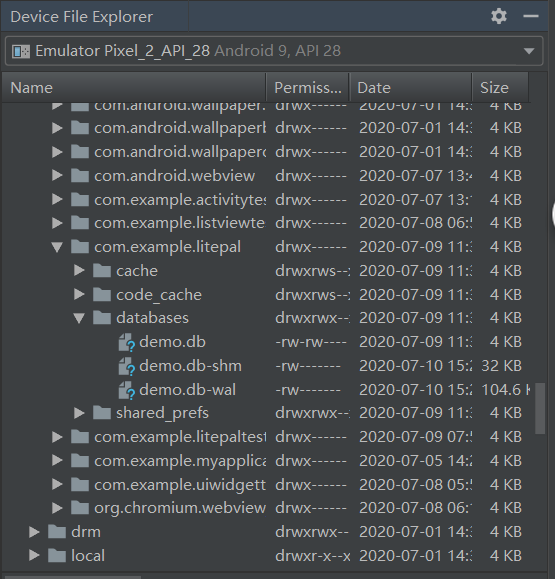
\includegraphics[width=0.4\textwidth]{database}
\caption{database} \label{database}
\end{figure}
我们可以去打开这个数据库,如图所示,Song表有两个表项,分别是我们上面在Song类中定义的name和duration:
\begin{figure}[H]
\small
\centering
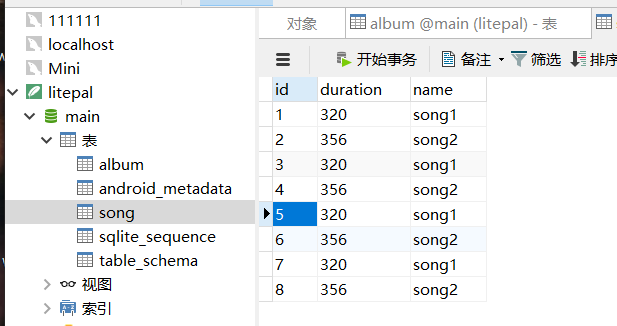
\includegraphics[width=0.4\textwidth]{table}
\caption{table} \label{table}
\end{figure}
\subsubsection{添加数据}
使用Litepal添加数据十分的简单,给人一种舒适的感觉.我们已经知道数据库中的Song表和我们前面定义的Song类是一一对应的,所以我们只需要在我们的MainActivity中新建一个Song对象,然后对该对象进行初始化,最后使用save()函数即可实现在数据库表中添加数据.MainActivity中的代码如下图所示:
\begin{lstlisting}[language=java]
package com.example.litepal;

import androidx.appcompat.app.AppCompatActivity;

import android.os.Bundle;
import android.util.Log;
import android.view.View;
import android.widget.Button;

import org.litepal.LitePal;

import java.util.List;

public class MainActivity extends AppCompatActivity {

    @Override
    protected void onCreate(Bundle savedInstanceState) {
        super.onCreate(savedInstanceState);
        setContentView(R.layout.activity_main);

        Button adddata = findViewById(R.id.add_data);
        adddata.setOnClickListener(new View.OnClickListener() {
            @Override
            public void onClick(View view) {

                Song song1 = new Song();
                song1.setName("song1");
                song1.setDuration(320);
                song1.save();

                Song song2 = new Song();
                song2.setName("song2");
                song2.setDuration(356);
                song2.save();
            }
        });
      
    }
}
\end{lstlisting}
这个save()方法是从哪里来的呢?还记得上面定义Song类继承了LitePalSupport类,那么这个save()方法就是该类中的方法,当你运行程序并且点击添加按钮时,song1和song2就会被添加到数据库中了,我们来看一下实际效果.
\begin{figure}[H]
\small
\centering
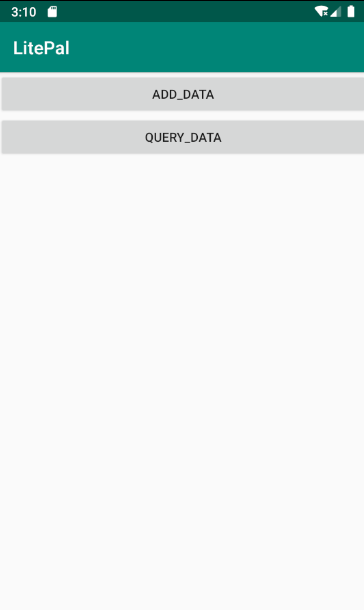
\includegraphics[width=0.4\textwidth]{run}
\caption{运行截图} \label{运行截图}
\end{figure}
\begin{figure}[H]
\small
\centering
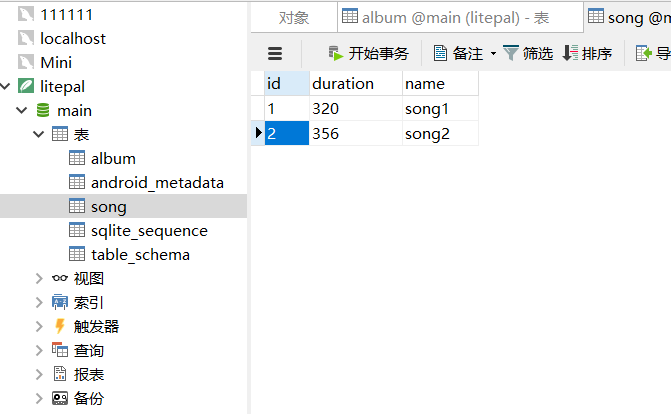
\includegraphics[width=0.4\textwidth]{addresult}
\caption{效果截图} \label{效果截图}
\end{figure}

\subsubsection{查询数据}
使用litepal查询数据一共有三种方式。

第一种方式:查询表中所有信息
\begin{lstlisting}[language=java]
List<Song> allSongs = LitePal.findAll(Song.class);
\end{lstlisting}

第二种方式:根据id查询表中某一行
\begin{lstlisting}[language=java]
Song song = LitePal.find(Song.class, id);
\end{lstlisting}

第三种方式:条件查询
\begin{lstlisting}[language=java]
List<Song> songs = LitePal.where("name like ? and duration < ?", "song%", "200").order("duration").find(Song.class);
\end{lstlisting}

为查看运行效果,我在MainActivity设置了一个按钮,用来查询Song表中的所有信息代码如下:
\begin{lstlisting}[language=java]
        Button lookdata = findViewById(R.id.query_data);
        lookdata.setOnClickListener(new View.OnClickListener() {
            @Override
            public void onClick(View view) {
                List<Song> allSongs = LitePal.findAll(Song.class);
                for(Song song:allSongs){
                    Log.d("MainActivity","Song's name is :"+song.getName());
                    Log.d("MainActivity","Song's duration is :"+song.getDuration());
                }
            }
        });
\end{lstlisting}
运行效果我是利用了Log函数,用来查看运行结果,下面是结果截图:
\begin{figure}[H]
\small
\centering
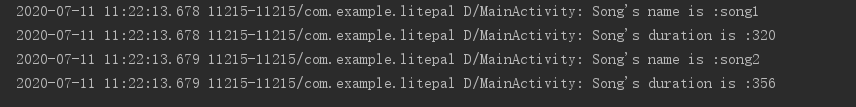
\includegraphics[width=0.4\textwidth]{query}
\caption{查询结果} \label{查询结果}
\end{figure}

\subsubsection{删除数据}
使用LitePal删除数据有两种方法。

第一种方法:删除表中的所有数据
\begin{lstlisting}[language=java]
LitePal.deleteAll(Song.class);
\end{lstlisting}

第二种方法:根据条件删除表格中的数据
\begin{lstlisting}[language=java]
LitePal.deleteAll(Song.class,"duration > ?","320");
//这一行也很简单,这行代码的意思是删除表格中duration>320的数据.
\end{lstlisting}

测试代码如下:
\begin{lstlisting}[language=java]
        Button deletedata = findViewById(R.id.delete_data);
        deletedata.setOnClickListener(new View.OnClickListener() {
            @Override
            public void onClick(View view) {
                // LitePal.deleteAll(Song.class);
                 LitePal.deleteAll(Song.class,"duration > ?","320");
            }
        });
\end{lstlisting}
运行结果截图:
\begin{figure}[H]
\small
\centering
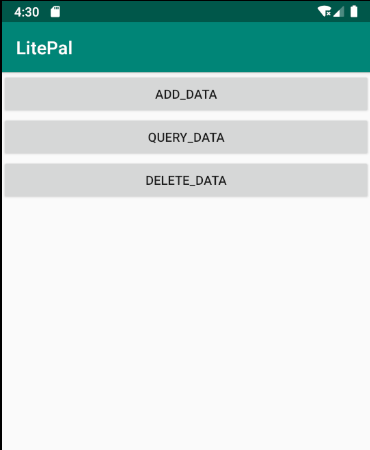
\includegraphics[width=0.4\textwidth]{delete}
\caption{运行界面} \label{运行界面}
\end{figure}

\begin{figure}[H]
\small
\centering
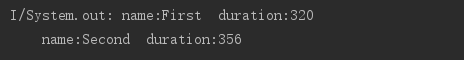
\includegraphics[width=0.4\textwidth]{delete1}
\caption{原始表} \label{原始表}
\end{figure}

\begin{figure}[H]
\small
\centering

\includegraphics[width=0.4\textwidth]{delete2}
\caption{删除后的表} \label{删除后的表}
\end{figure}


\subsubsection{更新数据}
LitePal数据库更新数据一共有以下几种方法,下面进行依次介绍。

第一种方法:这个是最简单的一种方法,首先通过find()函数来获取数据库表中的一行数据,也就是得到一个对象,然后对该对象进行数据变更操作,最后再使用save()函数保存即可.
\begin{lstlisting}[language=java]
Album albumToUpdate = LitePal.find(Album.class, 1);
albumToUpdate.setPrice(20.99f); // raise the price
albumToUpdate.save();
\end{lstlisting}

第二种方法:通过id更新数据库中的数据
\begin{lstlisting}[language=java]
Album albumToUpdate = new Album();
albumToUpdate.setPrice(20.99f); // raise the price
albumToUpdate.update(id);
\end{lstlisting}

第三种方法:这种方法是最常用的方法,即根据条件变更数据
\begin{lstlisting}[language=java]
Album albumToUpdate = new Album();
albumToUpdate.setPrice(20.99f); // raise the price
albumToUpdate.updateAll("name = ?", "album");
\end{lstlisting}
下面给出我的测试代码:
\begin{lstlisting}[language=java]
        Button update = findViewById(R.id.update_data);
        update.setOnClickListener(new View.OnClickListener() {
            @Override
            public void onClick(View view) {
                  Song newsong = new Song();
                  newsong.setDuration(999);
                  newsong.updateAll("name = ?","Five");
            }
        });
\end{lstlisting}
\begin{figure}[H]
\small
\centering
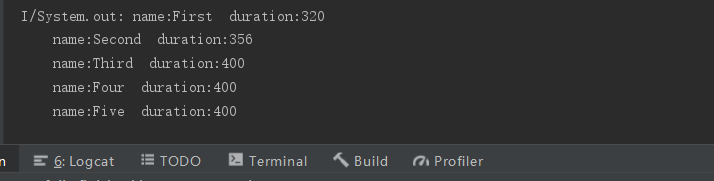
\includegraphics[width=0.4\textwidth]{update}
\caption{变更前的表} \label{变更前的表}
\end{figure}
\begin{figure}[H]
\small
\centering
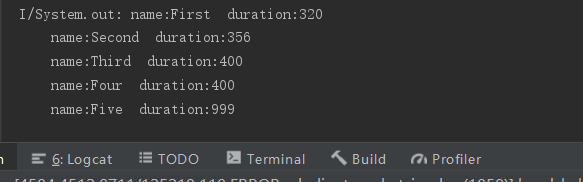
\includegraphics[width=0.4\textwidth]{update1}
\caption{变更后的表} \label{变更后的表}
\end{figure}
\subsection{实例总结}
在这里我把我实验使用的代码展示出来,并且通过ListView来展示数据库中的内容


第一个文件:类Song
\begin{lstlisting}[language=java]
package com.example.litepal;

import org.litepal.crud.LitePalSupport;

public class Song extends LitePalSupport {

    private String name;

    private int duration;

    public void setName(String s)
    {
        this.name=s;
    }

    public String getName()
    {
        return name;
    }

    public void setDuration(int s)
    {
        this.duration=s;
    }

    public int getDuration()
    {
        return duration;
    }

}
\end{lstlisting}

第二个文件:ListView针对Song类定义的适配器
\begin{lstlisting}[language=java]
package com.example.litepal;

import android.content.Context;
import android.view.LayoutInflater;
import android.view.View;
import android.view.ViewGroup;
import android.widget.ArrayAdapter;
import android.widget.TextView;

import java.util.List;
public class SongAdapter extends ArrayAdapter<Song> {
    private int resourceId;
    public SongAdapter(Context context, int textViewResourceId, List<Song> Objects) {
        super(context, textViewResourceId, Objects);
        resourceId = textViewResourceId;
    }
        public View getView(int position,View convertView , ViewGroup parent)
        {
             Song song = getItem(position);
             View view = LayoutInflater.from(getContext()).inflate(resourceId,parent,false);
             TextView songname=view.findViewById(R.id.song_name);
             songname.setText(song.getName());
             return view;
        }
}
\end{lstlisting}

第三个文件:数据库需要使用的litepal.xml文件
\begin{lstlisting}[language=xml]
<?xml version="1.0" encoding="utf-8"?>
<litepal>
    <dbname value="demo" />


    <version value="1" />


    <list>
        <mapping class="com.example.litepal.Album" />
        <mapping class="com.example.litepal.Song" />
    </list>

    -->

</litepal>
\end{lstlisting}

第四个文件:类MainActivity
\begin{lstlisting}[language=xml]
package com.example.litepal;

import androidx.appcompat.app.AppCompatActivity;

import android.os.Bundle;
import android.view.View;
import android.widget.Button;
import android.widget.ListView;

import org.litepal.LitePal;

import java.util.List;

public class MainActivity extends AppCompatActivity {
    private  List<Song>  SongList= LitePal.findAll(Song.class);

    @Override
    protected void onCreate(Bundle savedInstanceState) {
        super.onCreate(savedInstanceState);
        setContentView(R.layout.activity_main);
        Button adddata = findViewById(R.id.add_data);
        adddata.setOnClickListener(new View.OnClickListener() {
            @Override
            public void onClick(View view) {

                Song song1 = new Song();
                song1.setName("First");
                song1.setDuration(320);
                song1.save();

                Song song2 = new Song();
                song2.setName("Second");
                song2.setDuration(356);
                song2.save();

                Song song3 = new Song();
                song3.setName("Third");
                song3.setDuration(400);
                song3.save();

                Song song4 = new Song();
                song4.setName("Four");
                song4.setDuration(400);
                song4.save();

                Song song5 = new Song();
                song5.setName("Five");
                song5.setDuration(400);
                song5.save();
            }
        });
        Button lookdata = findViewById(R.id.query_data);
        lookdata.setOnClickListener(new View.OnClickListener() {
            @Override
            public void onClick(View view) {
                List<Song> allSongs = LitePal.findAll(Song.class);
                for(Song song:allSongs){
                   System.out.println("name:"+song.getName()+"  duration:"+song.getDuration());
                }
            }
        });
        Button deletedata = findViewById(R.id.delete_data);
        deletedata.setOnClickListener(new View.OnClickListener() {
            @Override
            public void onClick(View view) {
                 LitePal.deleteAll(Song.class);

            }
        });
        Button update = findViewById(R.id.update_data);
        update.setOnClickListener(new View.OnClickListener() {
            @Override
            public void onClick(View view) {
                  Song newsong = new Song();
                  newsong.setDuration(999);
                  newsong.updateAll("name = ?","Five");
            }
        });

        SongAdapter adapter = new SongAdapter(MainActivity.this,R.layout.song_item,SongList);
        ListView listview = findViewById(R.id.list_view);
        listview.setAdapter(adapter);


    }
}
\end{lstlisting}

第五个文件:activitymain.xml布局文件
\begin{lstlisting}[language=xml]
<?xml version="1.0" encoding="utf-8"?>
<LinearLayout xmlns:android="http://schemas.android.com/apk/res/android"
    android:orientation="vertical"
    android:layout_width="match_parent"
    android:layout_height="match_parent">
    <Button
        android:id="@+id/add_data"
        android:layout_width="match_parent"
        android:layout_height="wrap_content"
        android:text="add_data"
        />
    <Button
        android:id="@+id/query_data"
        android:layout_width="match_parent"
        android:layout_height="wrap_content"
        android:text="query_data"
        />
    <Button
        android:id="@+id/delete_data"
        android:layout_width="match_parent"
        android:layout_height="wrap_content"
        android:text="delete_data"
        />
    <Button
        android:id="@+id/update_data"
        android:layout_width="match_parent"
        android:layout_height="wrap_content"
        android:text="update_data"
        />
    <ListView
        android:id="@+id/list_view"
        android:layout_width="match_parent"
        android:layout_height="match_parent" />
</LinearLayout>
\end{lstlisting}

第六个文件:songitem.xml文件
\begin{lstlisting}[language=xml]
<LinearLayout xmlns:android="http://schemas.android.com/apk/res/android"
    android:layout_height="match_parent"
    android:layout_width="wrap_content">

    <TextView
        android:id="@+id/song_name"
        android:layout_height="wrap_content"
        android:layout_width="wrap_content"
        android:layout_marginLeft="10dp" />
</LinearLayout>
\end{lstlisting}

下面是运行效果截图:分别是四个按钮,以及一个展示数据库Song表的ListView
\begin{figure}[H]
\small
\centering
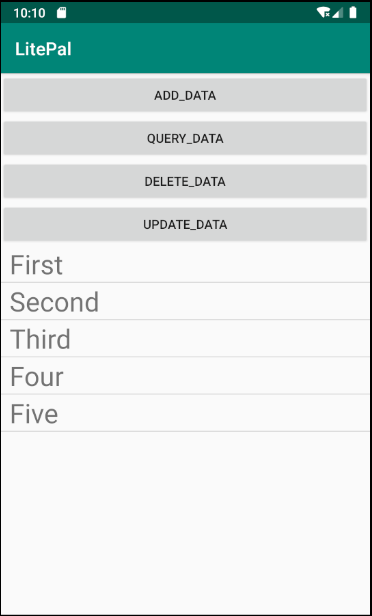
\includegraphics[width=0.4\textwidth]{result111}
\caption{效果实验效果} \label{实验效果}

\end{figure}
\subsection{总结}
LitePal是一款开源的Android数据库框架,采用对象关系映射(ORM)模式,将常用的数据库功能进行封装,可以不用写一行SQL语句就可以完成创建表、增删改查的操作。总的来说LitePal框架功能就是将自定义的类自动转换成内置数据库中的表,除此之外,它还把对数据库的原生语言操作变为了更简单的增删改查操作,LitePal是一个容易掌握,简洁轻便的Android内置数据库框架,推荐使用~~



%===参考文献===
%\addcontentsline{toc}{section}{参考文献}
%\bibliographystyle{abbrv}     %论文引用格式
%\bibliography{E:/studio/write/bibkit/wholebiblio}
                         
\begin{thebibliography}{99}
\bibitem{A19}
{\em \color{red}官方文档}. \url{https://github.com/guolindev/LitePal}, 2020.

\bibitem{B19}
{\em \color{red}《第一行代码》<郭霖>}.
\end{thebibliography}
\end{document}
%===结束===



